\documentclass[../main.tex]{subfiles}
\begin{document}

\section{Board Setup}
Here we will walk through the different steps of setting up the board. Keep in mind that players can customize their maps in terms of size, elevation, roads, materials, and other factors to achieve the gameplay experience that best fits the preferences of their group.
\begin{figure}[h]
    \centering
    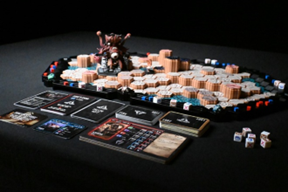
\includegraphics[width=1\linewidth]{boardsetup1.png}
\end{figure}

\subsection{Step 1:  Place the edges}
Place and interlock the Edges to create the play area of the board.

\begin{figure}[h]
    \tsgap
    \centering
    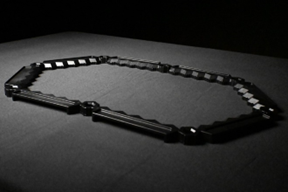
\includegraphics[width=1\linewidth]{boardsetup_edges.png}
\end{figure}

The Edges of the board are used to define the boundaries of the game and to hold the dice and markers. Feel free to play with the angles of the Edges to build many different shapes and sizes.

\textit{Recommendation: We recommend using eight Edges for 2-5 player games.}

\subsection{Step 2:  Fill in the Base Layer}
Place a base layer of basic land hexes (sand) for Characters to move on.

\begin{figure}[h]
    \tsgap
    \centering
    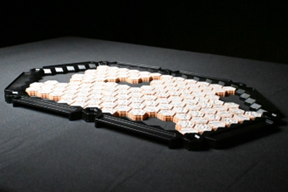
\includegraphics[width=1\linewidth]{baselayer.png}
\end{figure}

The base layer of the board is the foundation of the game and cannot be changed by the Sentience or other effects.

\textit{Recommendation: Use the larger hexes to help build the base layer faster.}

Place water or lava tiles to create lakes, rivers, and other liquid traps and hazards. 

\begin{figure}[h]
    \tsgap
    \centering
    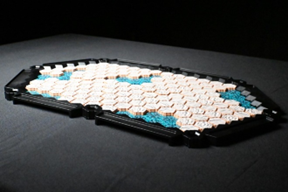
\includegraphics[width=1\linewidth]{chapters//boardsetup/watersetup.png}
\end{figure}

Access to water is important to gameplay and is required to perform actions like Fishing.

\clearpage
\subsection{Step 3:  Add Elevation and More}
Place additional basic land hexes (sand) to create height.

\begin{figure}[h]
    \centering
    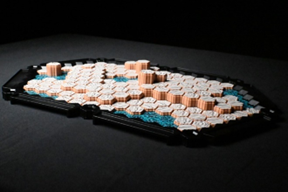
\includegraphics[width=1\linewidth]{chapters//boardsetup/sandplacement.png}
\end{figure}

Elevation is a feature that can impact strategic play and is subject to destruction during the game.

Roads and walls can also be added to the setup of the board but are also able to be built during gameplay.

\subsection{Step 4:  Place Resources}
Place resource hexes (obsidian or red rock) around the board.

\begin{figure}[h]
    \centering
    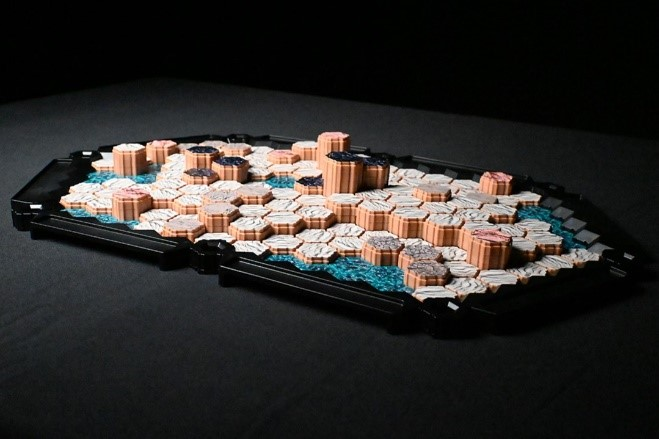
\includegraphics[width=1\linewidth]{chapters//boardsetup/TimeStrikePlaceResources.jpg}
\end{figure}

Materials are gathered from resource hexes by Characters and used to build walls and roads. When placing resource hexes, we suggest placing some in easy-to-reach areas, and others in difficult-to-reach areas, such as high mountain peaks. 

\textit{Recommendations: We recommend placing approximately five resource hexes per player. }

\subsection{Step 5:  Set up Card Area}
Create an area to place the multiple decks of cards. Players will be drawing from and referencing cards in this area throughout the game. Locate the loot, fish, and quest card decks. Shuffle each deck individually, then place each deck face down in the card area.

\begin{figure}[h]
    \centering
    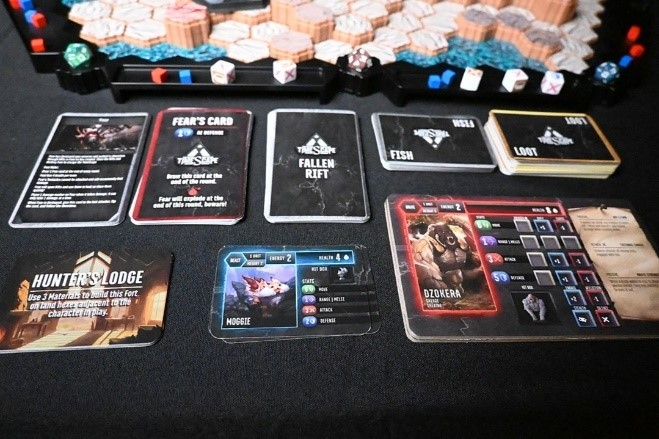
\includegraphics[width=1\linewidth]{chapters//boardsetup/TimeStrikeCardPlacement.jpg}
\end{figure}

Search through the Character cards to find the ones labeled "Monster-Brute", remove them from the Character card deck and place them in a separate pile.

\begin{figure}[h]
    \centering
    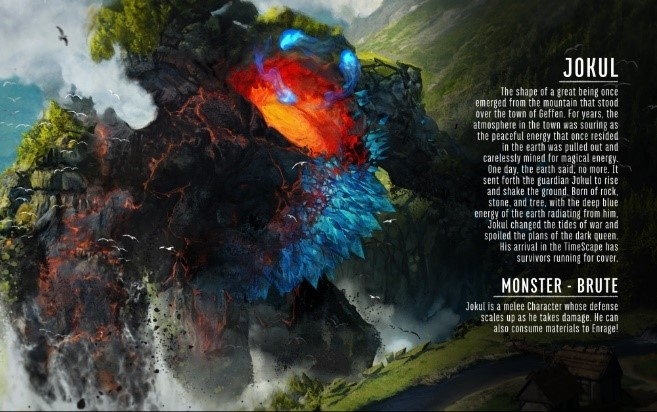
\includegraphics[width=1\linewidth]{chapters//boardsetup/TimeStrikeCharacterCardMonster.jpg}   
\end{figure}

Locate the Sentience card deck and set aside all three cards that have a red border. Shuffle the remaining Sentience cards and place the deck face down. Pick up one red bordered Sentience card on top of the shuffled deck, count down the deck three cards, place the second red bordered Sentience card, count down the deck three more cards, and place the third red bordered Sentience card. 

\clearpage

From top of the deck to the bottom the deck should look like: Red - Gray- Gray- Gray - Red - Gray- Gray- Gray - Red - Gray- Gray- Gray. 
\begin{figure}[h]
    \centering
    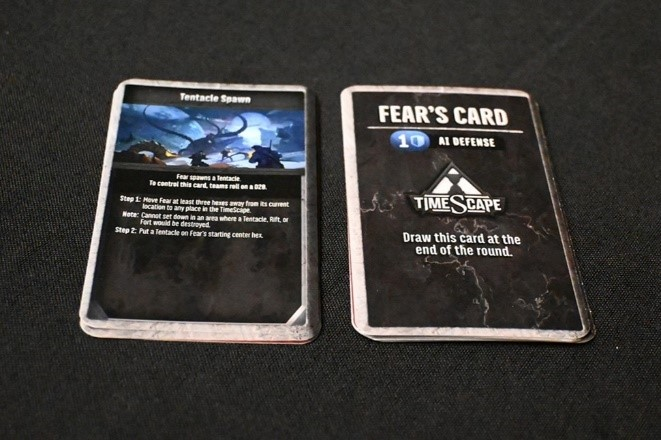
\includegraphics[width=1\linewidth]{chapters//boardsetup/TimeStrikeSentienceCards.jpg}
\end{figure}

\subsection{Step 6:  Place the Sentience, Mobs, and Monsters}
The following setup is specific to setting up the Sentience: Fear. 
\begin{figure}
    \centering
    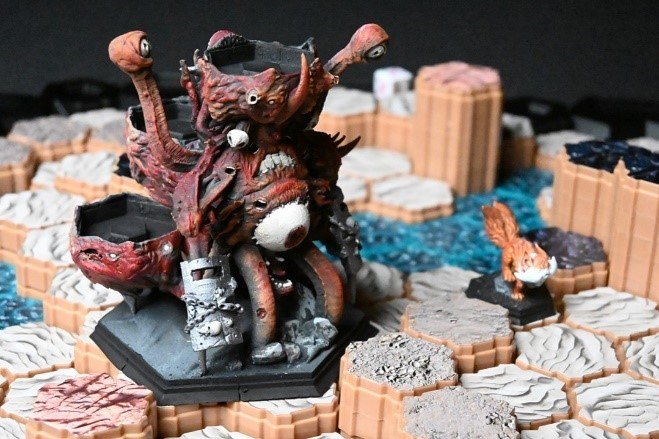
\includegraphics[width=1\linewidth]{chapters//boardsetup/TimeStrikeSentienceFearMini.jpg} 
\end{figure}
Fear and it's Monsters (referred to as the Lost) are threats that can be battled to help Characters progress. 
\begin{enumerate}
    \item Place the Fear miniature anywhere on the board that it fits. The base should be supported by a flat surface of at least five hexes. The Sentience takes up a total space of seven hexes, but can be left with up to two hexes unsupported. 
    \textit{Recommendation: Place the Sentience near the center of the board for ideal game play. }
    \item Place one of the Fear's tentacles anywhere on the board. 
    \textit{Note: For a more threatening boss, start with more tentacles. }
    \item Place your Beasts. The number of Beasts is determined by the number of players. Refer to the chart below for additional players. 
    
    \begin{table}[h]
        \centering
        \begin{tabular}{ccc}
             1 - 2 Players  & 3 - 4 Players & 5 - 6 Players\\
             1 Beast & 2 Beasts  & 3 Beasts \\
        \end{tabular}
    \end{table}
    
    Then locate the corresponding Beasts cards and place then facing up to show that they are active. Place the remaining unused Beast cards aside in a separate pile. 
    
    \begin{figure}[h]
        \centering
        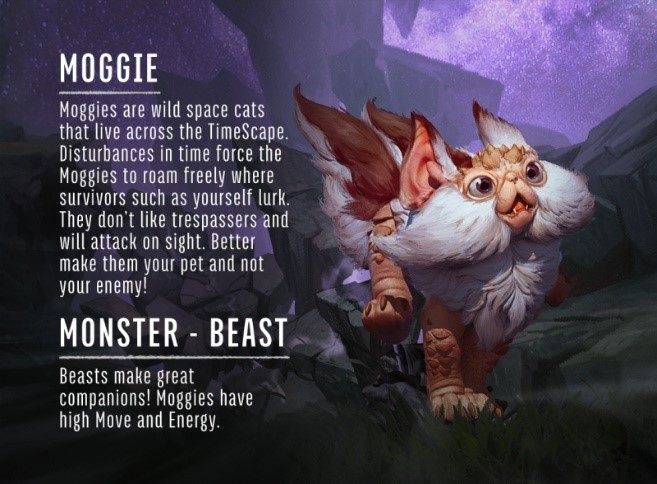
\includegraphics[width=1\linewidth]{chapters//boardsetup/TimeStrikeBeastCard.jpg}
    \end{figure}
    
\end{enumerate}
\clearpage

\end{document}
